\documentclass{article}

\usepackage[numbers]{natbib}
\usepackage[utf8]{inputenc} % allow utf-8 input
\usepackage[T1]{fontenc}    % use 8-bit T1 fonts
\usepackage{hyperref}       % hyperlinks
\usepackage{url}            % simple URL typesetting
\usepackage{booktabs}       % professional-quality tables
\usepackage{amsfonts}       % blackboard math symbols
\usepackage{nicefrac}       % compact symbols for 1/2, etc.
\usepackage{microtype}      % microtypography

%%------
%% add customized lines here:

\usepackage{makecell}
\usepackage{multirow}
\usepackage{pbox}
\usepackage{multicol}
\usepackage[toc,page]{appendix}
\usepackage{amsfonts}
\usepackage{amsmath}
\usepackage{graphicx}
\usepackage{caption}
\usepackage{subcaption}
\usepackage{float}
\usepackage{hyperref}
\usepackage{listings}
\usepackage{algorithm}
\usepackage[noend]{algpseudocode}
%\usepackage{pdfsync}
\usepackage{color}

\title{Probability Amplitude Based Neural Networks}
\author{elem6}

\date{}
\begin{document}

\maketitle
\begin{abstract}
  We propose a new type of neural networks inspired by the path integral
  formulation of quantum mechanics. Current models of neural networks use a
  linear function as the link between neurons in different layers, and the
  non-linearity is provided by the activation function. We show that it is
  possible to replace the linear link between two neurons with a non-linear
  complex function called probability amplitude in quantum
  mechanics. Empirically, fully connected probability amplitudes based
  neural networks generalize comparably with other types of fully connected
  neural networks.
\end{abstract}

\section{Introduction}

The capability of universal approximation~\cite{cybenko, hornik, leshno,
  sonoda} is one of the key reasons that deep neural
networks~\cite{deeplearning} perform so well. The commonly used connections
between neurons in different layers are as follows. A given computing unit
(neuron) in a hidden layer takes as input the affine transformation of the
outputs of neurons in the lower layer, and outputs the value of its
activation function \(f\) of the form
\begin{equation}
  \label{eq:affine}
  x^{l}_{\alpha} = f\left(\sum_{\beta} w^{l}_{\alpha\beta}x^{l-1}_{\beta} + b^{l}_{\alpha}\right),
\end{equation}
where \(x^{l}_{\alpha}\) is the output of \(\alpha\)-th neuron in \(l\)-th
layer. \({\bf w}^{l}\) and \({\bf b}^{l}\) are weights and biases,
respectively. To distinguish neuron indices from layer indices and the
imaginary unit \(i\), we use Greek letters to denote neurons. There are
several popular choices for the activation function \(f\), such as the
logistic sigmoid (\(\sigma\)), hyperbolic tangent function
(tanh)~\cite{tanh}, and rectified linear unit (ReLU)~\cite{relu,
  deep_sparse}. 

Beside affine functions, a neural network can also use radial basis
functions~\cite{broomhead, park} as connections between neurons in different
layers. In this type of networks, each hidden node acts as a centroid with
coordinate \(\bf c\), and its activation function is a function of the
distance (not necessarily the Euclidean metric) between the input \(\bf x\)
and \(\bf c\), namely,
\begin{equation}
  \label{eq:rbf}
  x_{\alpha}^{l} = \lambda_{\alpha}\phi\left(\frac{\|{\bf x}^{l-1} - {\bf c}_{\alpha}\|}{\sigma_{\alpha}}\right).
\end{equation}
Usually \(\phi\) is taken to be a Gaussian function.

Mathematically, the aforementioned networks are all universal approximators.
They can be trained to construct functions that fit a training set
arbitrarily well. This is true even for randomly labeled training set simply
because having enough parameters, the network can memorize all the training
data~\cite{zhang}. However, different networks have different
generalizations when used as classifiers on the test set. Furthermore, when
applying backpropagation to train the networks, different activation
functions perform differently since backpropagation relies heavily on the
properties of the gradient of the activation functions~\cite{glorot}. Due to
the above reasons, finding new types of connections between
neurons~\cite{maas, he, xu, elu, capsnet, unitary, minemoto, dqn, dcn} is an
active research area.

In this work, we propose a type of neural networks based on probability
amplitude (henceforth PaNet) which is inspired by the path integral
formulation~\cite{feynman} of quantum mechanics. In the following, we give a
detailed description of how to construct the network, and show some of its
applications. To limit the scope, we will only consider fully connected
networks.

\section{Structure of  PaNet}

A PaNet is similar to other neural networks. It consists of an input layer,
an output layer, and one or more hidden layers. The difference lies in how
neurons in different layers being connected. More generally, a PaNet is a
layered directed graph. Associated with each edge \(\beta \to \alpha\) of
the graph, we define a complex link function
\begin{equation}
  \label{eq:link}
  \Gamma^{l}_{\alpha\beta} = \exp\left\{i(w^{l}_{\alpha\beta}x^{l-1}_{\beta} + b^{l}_{\alpha\beta})\right\}.
\end{equation}
As before, \(l\) is the layer index, \(x^{l-1}_{\beta}\) is the output from
vertex \(\beta\). \(w^{l}_{\alpha\beta}\) and \(b^{l}_{\alpha\beta}\) are
the scale and shift factors that can be determined by a learning algorithm,
which are similar to the weights and biases of a traditional neural
networks. A vertex (neuron) of the graph is the basic computing unit which
takes as arguments the incoming links, and computes a real or complex value
according to its activation function:
\begin{equation*}
  x_{\alpha}^{l} = f\left(\sum_{\beta}\Gamma^{l}_{\alpha\beta}\right).
\end{equation*}
To limit the scope, we only consider the following types of activation function,
\begin{equation}
  \label{eq:af}
  x_{\alpha}^{l} = f\left(\left\|\frac{1}{\mathnormal{N}}\sum_{\beta}\Gamma^{l}_{\alpha\beta}\right\|^{2}\right),
\end{equation}
where we introduced a normalization constant \(\mathnormal{N}\).
\begin{figure}[htb]
  \centering
  % 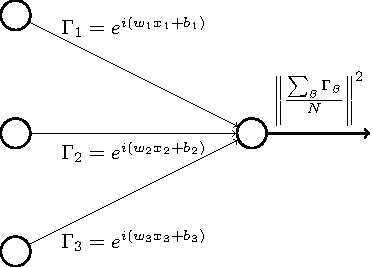
\includegraphics[width=0.5\textwidth]{links}
  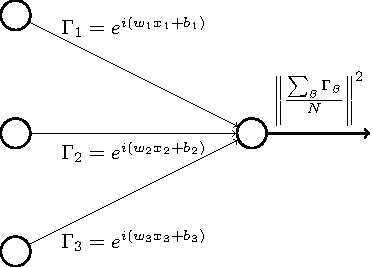
\includegraphics{links}
  \caption{A simple neural network based on probability amplitude. }
  \label{fig:Network}
\end{figure} 
In Figure \ref{fig:Network}, a neuron on the right is shown to be linked to
three other neurons on the left with links \(\Gamma_{\beta}\)'s, where
\(\beta = 1, 2, 3\). Its activation is the squared modulus of the normalized
sum of the links.

The complex function \(\Gamma^{l}_{\alpha\beta}\) is called probability
amplitude in quantum mechanics. It is so called because in the context of
path integral formulation, the squared modulus
\(\|\Gamma^{l}_{\alpha\beta}\|^{2}\) is proportional to the probability
distribution of a physical observable such as position or momentum. For
example, we can imagine a particle moves through a three-layer network
starting from vertex \(\beta\) in the first layer, the probability of
finding it at vertex \(\alpha\) in the third layer is
\begin{equation*}
  P_{\alpha\beta} \propto \left\| \sum_{\gamma}\Gamma^{3}_{\alpha\gamma}\Gamma^{2}_{\gamma\beta}\right\|^{2}.
\end{equation*}
We will, however, not use this sum over paths formulation. We will stick to
the activation function in Eq.~\ref{eq:af} where computation is done layer
by layer so that the standard backpropagation can be applied to train the
network. 

\section{Properties}

Classification, an important application of neural networks, is essentially
a process of reducing redundant information. For example, the
MNIST~\cite{MNIST} data set consists a set of images of handwritten digit and
their labels. The images have a size of 784 (\(28\times28\)) pixels. The
goal is to classify the test images to digits. A neural network for
classifying the data set can be thought as consisting 10 distinctive
functions, each is constructed to recognize one of the digits. Suppose we
normalize the images so that the value of each pixel lies in \([0,1]\), then
these functions are mappings from \(D\)-dimensional unit cube \([0, 1]^{D}\)
to \([0,1]\), where \(D = 784\). Knowing the location and intensity of a
particular pixel in an image will not provide much information about what
the digit is. This implies that the image contains a lot of redundant
information. The redundancy comes at least from: 1) large portion of the
pixels come from the uniform background of the images; 2) for a given digit,
the handwritten images varies both in the number of bright pixels and the
locations/intensities of these pixels. It is the local correlations among
the pixels at certain length scales that determine which digit they
represent. For example, instead of full connections between layers,
convolutional neural networks~\cite{convnet} use local receptive fields to
extract features and result in much better accuracy.

Thus, to be effective, functions constructed by training a network 1) must
not change for certain variations of the input so as to remove redundancy,
and 2) should change when some combinations of pixels are present so as to
detect correlations. We can visualize how affine function
\(y(\mathbf{x}) = \mathbf{w}^{T}\mathbf{x} + b\) achieves these two things
by noting that, for a fixed \(y = y_{0}\), the equation
\(\mathbf{w}^{T}(\mathbf{x} - \mathbf{x}_{0})= 0\) defines a plane \(S\) in
\(\mathbb{R}^{D}\), where \(\mathbf{w}^{T}\mathbf{x}_{0} = y_{0} - b\). For
all \(\mathbf{x} \in S\), the value \(y\) of the affine function does not
change. On the other hand, if \(\mathbf{x}\) grows along the direction of
\(\mathbf{w}\), the value \(y\) will achieve the maximum change since
\(\mathbf{w}\) is the gradient of the affine function. Thus the gradients
are related to correlations.

\begin{figure}[htb]
  \centering
  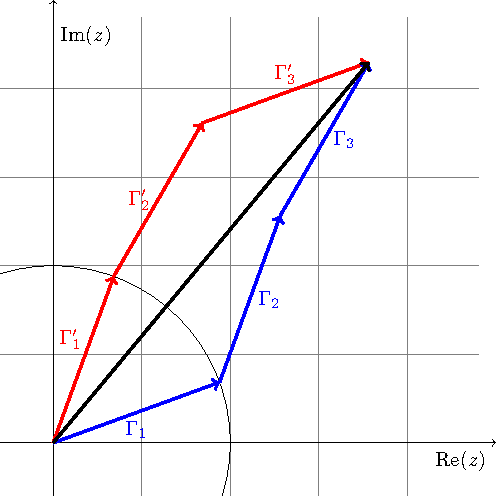
\includegraphics[width=0.4\textwidth]{sum}
  \caption{Sum of probability amplitudes. Two different sets of probability
    amplitudes may have the same sum.}
  \label{fig:sum}
\end{figure}

Now let us look at how PaNet achieve these two things. Consider the sum of
probability amplitudes
\begin{align}
  \label{eq:summation}
  z = \sum_{\alpha=1}^{D}\Gamma_{\alpha}(x_{\alpha}),
\end{align}
where \(\Gamma_{\alpha}(x_{\alpha}) = e^{i\varphi_{\alpha}(x_{\alpha})}\)
and \(\varphi_{\alpha}(x_{\alpha}) = w_{\alpha}x_{\alpha} + b_{\alpha}\) as
defined in Eq.~\ref{eq:link} but with output neuron indices and layer
indices suppressed. In the complex plane, each \(\Gamma_{\alpha}\) is a unit
vector. When all the unit vectors point to the same direction, the modulus
of the sum is maximized, with \(\mathrm{sup}\ \|z\| = D\). If all the
vectors are evenly spaced on the unit circle, the sum reaches zero, namely,
\(\mathrm{inf}\ \|z\| = 0\). In between these two bounds, the more the
vectors align, the larger the modulus becomes. As shown in
Fig.~\ref{fig:sum}, there are many arrangements for the vectors that have
the same sum so that the modulus is invariant for these inputs. In the
parlance of physics, these probability amplitudes can either interfere
constructively or destructively. For example, the squared modulus of the sum
of two probability amplitudes is
\begin{align*}
\|\Gamma_{1}+ \Gamma_{2}\|^{2} = 2(1 + \cos(\varphi_{1} - \varphi_{2})).
\end{align*}
When \(\Gamma_{1}\) and \(\Gamma_{2}\) are in phase
(\(\varphi_{1} - \varphi_{2} = 0\)), the squared modulus is 2; when they are
out of phase (\(\varphi_{1} - \varphi_{2} = \pi\)), it is 0.

As for the activation function in Eq.~\ref{eq:af}, the simplest function one
may use is \(\|z/D\|^{2}\). Explicitly, the activation is
\begin{align}
  \label{eq:smod}
  \rho(\mathbf{x}) &= \left\|\sum_{\alpha=1}^{D}\frac{\Gamma_{\alpha}(x_{\alpha})}{D}\right\|^{2} \nonumber \\
                   &= \frac{2}{D^{2}}\sum_{\alpha < \beta}\cos(w_{\alpha}x_{\alpha} + b_{\alpha} - w_{\beta}x_{\beta} - b_{\beta}) + \frac{1}{D}.
\end{align}
Note that \(\rho(\mathbf{x})\) is a sum of functions of two variables, its
value depends on the pairwise phase differences of the probability
amplitudes. 

One interesting property of PaNet is that in general it requires at least
two hidden layers to work. This is related to the problem of representing or
approximating a continuous function \(f: [0,1]^{D} \to [0,1]\) by
superposition of functions with a small number of
variables~\cite{kolmogorov,arnold, hecht-nielsen}. Using probability
amplitudes, we can approximate the function with
\begin{align}
  \label{eq:two-layers}
  f(\mathbf{x}) &= \left\|\frac{1}{N}\sum_{\beta = 1}^{N}\Gamma_{\beta}
                  \left(\rho_{\beta}(\mathbf{x})\right)\right\|^{2},
\end{align}
where \(\rho_{\beta}(\mathbf{x})\) is defined in Eq.~\ref{eq:smod}, and
\(N\) is an integer we can choose to achieve the accuracy we
need. Intuitively, as pointed out by Arnold~\cite{arnold}, we can understand
the two-layer structure by the concept of the tree of components of level
sets of the function \(f\). A level set of a function is the set of points where
the function takes a fixed value. The level set may consists one or several
connected components. And the level sets can be thought as organized in a
tree structure. This is similar to what we have described above that a
neuron must be trained to be insensitive to certain sets of inputs, and
sensitive to other sets of inputs. The two-layer superposition works as
follows. The inner functions map the domain of the function \(f\) to the
tree of components of the level sets, the outer functions map the components
to the segments that form the range of the function. It is worth stressing
that affine function based neural networks work in the same way, the function
can be approximated by~\cite{cybenko}
\begin{align}
  f(\mathbf{x}) = \sum_{\beta=1}^{N}c_{\beta}\sigma\left(\mathbf{w}^{T}_{\beta}\mathbf{x} + b_{\beta}\right),
\end{align}
where the affine function
\(\mathbf{w}_{\beta}^{T}\mathbf{x} + b_{\beta}\) plays the role of
\(\rho_{\beta}(\mathbf{x})\).

\section{Experiments}

The simplest yet nontrivial problem is probably the XOR (exclusive-or)
function, where we require \(f(1,0) = f(0,1) = 1, f(0,0) = f(1,1) = 0\). We
use the four data points to train both PaNet and the fully connected neural
network with tanh activation function (FCN), the results are shown in
Fig.~\ref{fig:xor}. Without surprise both networks can satisfy the
requirements quite well. Beyond these four points, they have very
interesting differences. XOR function approximated by PaNet features large
flat regions near these four points, and has sharper transitions between
high plateaus and low plains. The function approximated by FCN has more
gradual changes between different regions. Given their different behaviors,
one may find one of them is more suitable for certain problems than the
other, depending on the problem domain. It will be interesting to see
how PaNet performs in function interpolation problems.

\begin{figure}[t!]
  \centering
  \begin{subfigure}[t]{0.5\textwidth}
    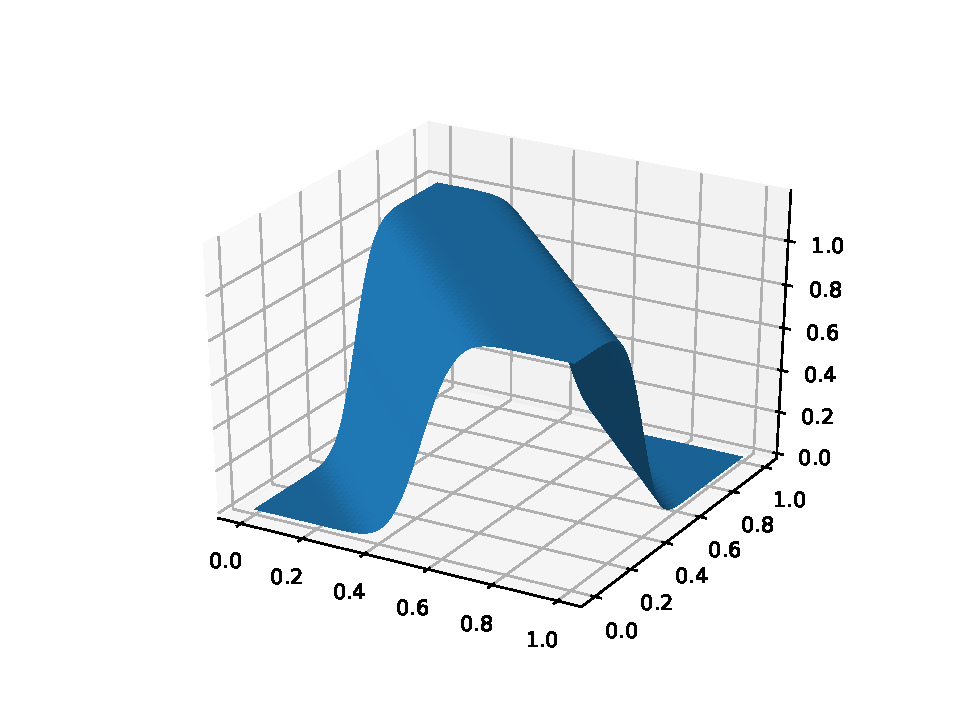
\includegraphics[trim={1cm 1cm 1cm 1cm},width=\textwidth,clip]{xor_panet}
    \caption{}
  \end{subfigure}%
  ~
  \begin{subfigure}[t]{0.5\textwidth}
    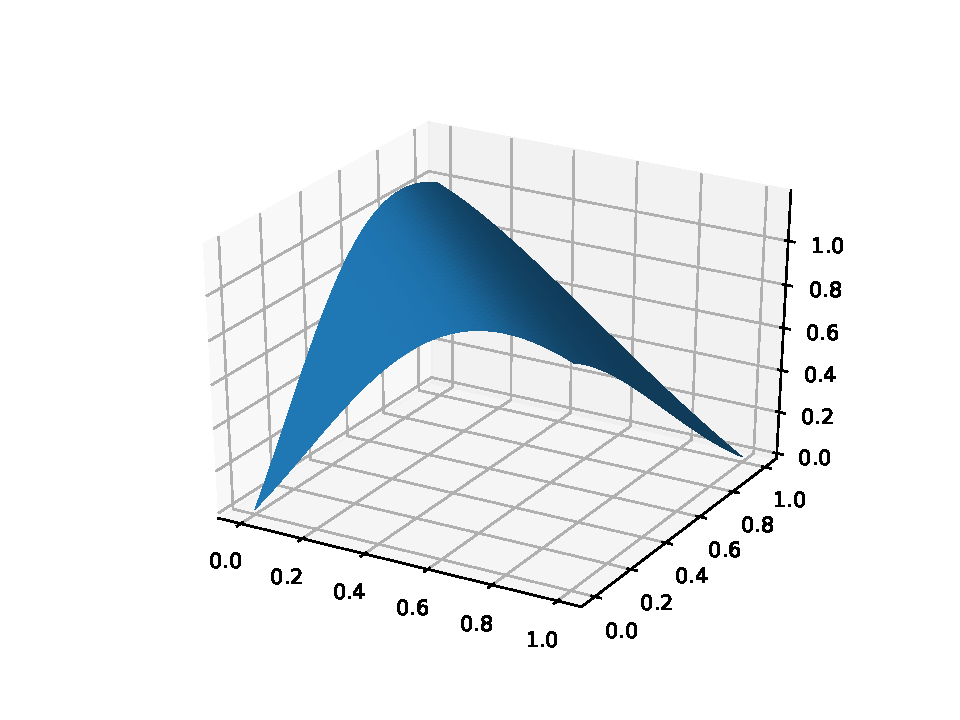
\includegraphics[trim={1cm 1cm 1cm 1cm},width=\textwidth,clip]{xor_affine_tanh}
    \caption{}
  \end{subfigure}
  \caption{XOR function approximated by networks trained using (a)
    probability amplitudes and (b) affine functions with hyperbolic tangent
    activation function.}
  \label{fig:xor}
\end{figure}

To see how PaNet generalizes, we used MNIST data set to test its
capability. To have a better result, we introduce the function
\begin{align}
  \label{eq:corr2var}
  \tilde{\rho}(x_{1}, x_{2}) = 2\left\|\frac{\Gamma_{1}(x_{1}) + \Gamma_{2}(x_{2})}{2}\right\|^{2} - 1,
\end{align}
so that when the two vectors are in phase, \(\tilde{\rho} = 1\), and when they are
out of phase, \(\tilde{\rho} = -1\). In general, for \(D\)-dimensional space, we can
define
\begin{align}
  \label{eq:corr}
  \tilde{\rho}(\mathbf{x}) &= 2\left\|\frac{\sum_{\alpha = 1}^{D}\Gamma_{\alpha}(x_{\alpha})}{D}\right\|^{2} - 1 \nonumber \\
                           &= \frac{4}{D^{2}}\sum_{\alpha < \beta}\cos(w_{\alpha}x_{\alpha} + b_{\alpha} - w_{\beta}x_{\beta} - b_{\beta}) + \frac{2}{D} - 1.
\end{align}
It can be verified numerically that the network performs better and
converges faster when using \(\tilde{\rho}\) as the output of the neuron
than using \(\rho\) defined in Eq.~\ref{eq:smod}. Note that the gradient for
a given parameter is a sum of \(D - 1\) terms, this might help avoiding the
vanishing gradient problem. Furthermore, since \(\mathbf{x}\) is confined in
\([0,1]^{D}\) and the derivatives with respect to the parameters is always
finite, the gradient will not explode either.

\begin{table}
    \caption{Results for test accuracy in percentage using different networks
      with different sizes for the MNIST data set.\\}
    \centering
  \begin{tabular}{l l l l l l l l l l}
    \toprule
    Network & \multicolumn{9}{c} {Number of Neurons in the Hidden Layer(s)} \\ \hline
            & 200    & 300     & 400     & 500     & 600     & 700    & 800    & 900    & 1000 \\
    \hline
    ReLU  & 98.27 & 98.38  & 98.44  & 98.53  & 98.49  & 98.56 & 98.48 & 98.55 & 98.60 \\
    tanh  & 98.15 & 98.31  & 98.25  & 98.34  & 98.25  & 98.30 & 98.34 & 98.24 & 98.26 \\
    PaNet & 98.17 & 98.20  & 98.31  & 98.35  & 98.43  & 98.36 & 98.46 & 98.50 & 98.50 \\
    \bottomrule
  \end{tabular}

  \label{tb:acc}
\end{table}

As discussed previously, PaNet with two hidden layers is mathematically
equivalent to affine function based networks with one hidden layer. In fact,
PaNet with one hidden layer will not be able to converge on the training
set. To determine its performance, we compared PaNet with two other
networks. The PaNet consists two hidden layers, and with mean squared error
as the cost function. The latter two networks have one hidden layer with
ReLU and tanh as activation function, respectively. We also applied softmax
activation function to the output layer, and used cross entropy as the cost
function. For each type and size of the networks, several runs were
performed. The best results for test accuracy are shown in
Table~\ref{tb:acc}. Within these results, PaNet is comparable with tanh
network when the number of neurons in the hidden layer is small, and is
comparable with ReLU network when the number of neurons in the hidden layer
increases. Loosely speaking, its generalization capability is somewhat
between tanh network and ReLU network.

\section{Conclusion}
\label{sec:conclusion}
In this paper, we proposed a new type of neural networks inspired by the
path integral formulation of quantum mechanics where neurons are connected
by probability amplitudes. Instead of a superposition of functions of one
variable to approximate a function of multiple variables, PaNet uses
essentially a superposition of functions of two variables in a pairwise
fashion. From a limited first impression, one disadvantage is that it needs
more parameters and layers to achieve an equivalent generalization in the
case of fully connected networks. However, we would like to stress that we
only considered some very narrow use cases, its full potential is still
awaiting further explorations. For example, it will be interesting to adapt
PaNet to convolutional neural networks or recurrent neural
networks~\cite{rnn}. Its unique way of linking neurons may lead to novel
structures in neural networks, and its mathematical structure may shed light
on how neural networks generalize.


\bibliography{References}
\bibliographystyle{plainnat}

\end{document}

%%% Local Variables:
%%% mode: latex
%%% TeX-master: t
%%% End:
